%%%%%%
%
% $Autor: Wings $
% $Datum: 2020-01-18 11:15:45Z $
% $Pfad: WuSt/Skript/Produktspezifikation/powerpoint/ImageProcessing.tex $
% $Version: 4620 $
%
%%%%%%

\chapter{Neuronale Netze}

Während Computer dem Menschen auf vielen Gebieten überlegen sind, gibt es dennoch Aufgaben, die ein Mensch auf Grund seiner Intelligenz und Lernfähigkeit intuitiv lösen kann, während eine Übertragung dieser  Fähigkeiten auf den Computer eine große Herausforderung darstellt. Ein populärer Ansatz zur Entwicklung  künstlicher Intelligenz liegt in künstlichen neuronalen Netzen (engl. artificial neural networks). Diese sind  \glqq informationsverarbeitende Systeme, deren Struktur und Funktionsweise dem Nervensystem und  speziell dem Gehirn von Tieren und Menschen nachempfunden sind\grqq.\cite{Kruse:2015}

Neuronale Netze bestehen - gemäß ihrem Namen - aus Neuronen, welche miteinander verbunden sind und sich gegenseitig beeinflussen. Die modellierten Neuronen können, wie ihr biologisches Vorbild, bei ausreichender Stimulation durch ein oder mehrere Eingangssignale aktiviert werden. Das biologische 
Neuron kann mit einem Kondensator verglichen werden, der durch kleine elektrische Spannungsimpulse 
von anderen Neuronen aufgeladen wird. Überschreitet die so erreichte Spannung einen Schwellwert, 
gibt das Neuron selbst einen Spannungsimpuls an verbundene Neuronen weiter. Dieses Prinzip wird in 
künstlichen neuronalen Netzen durch mathematische Modelle nachgeahmt. Abbildung \ref{NNBio} zeigt 
die erste Abstrahierungsstufe von biologischen neuronalen Netzen hin zu den mathematischen Modellen. 
\cite{Ertel:2016}

\begin{figure}[H]
	\begin{center}
		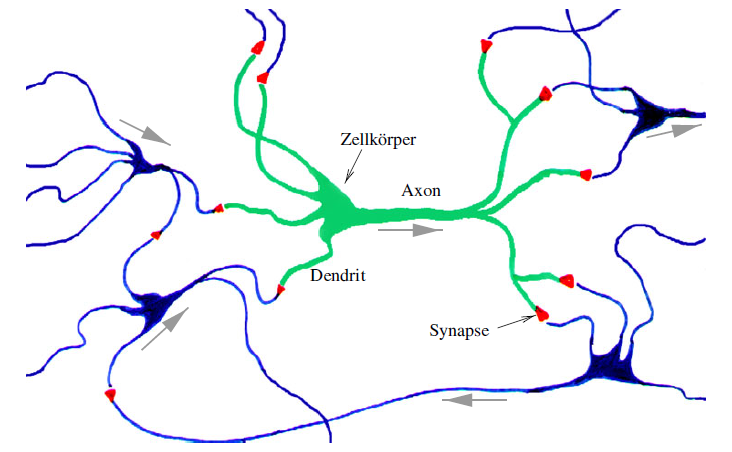
\includegraphics[width=0.49\textwidth]{NeuralNetwork/NeuronBio}
		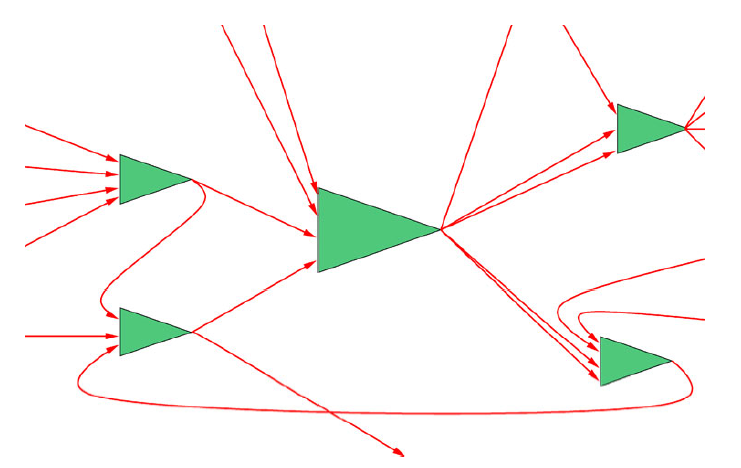
\includegraphics[width=0.49\textwidth]{NeuralNetwork/NeuronAbstrakt}
		\caption{Biologisches (links) und abstrahiertes (rechts) Modell neuronaler Netze. Quelle:\cite{Ertel:2016}} 
		\label{NNBio}
	\end{center}
\end{figure}

1958 stellt Frank Rosenblatt die einfachste Form eines neuronalen Netzes vor. Dieses, als
einlagiges Perzeptron vorgestellte Modell, enthält eine Schicht von Eingabeneuronen, die
alle mit einem Ausgangsneuron verbunden sind. \cite{Dorn:2018} Sind mehrere Neuronen schichtweise 
hintereinandergeschaltet, ist die Rede vom mehrlagigen Perzeptron. Die Ausgabe
eines Neurons fungieren dabei als Eingangssignal für das nachfolgende Neuron, bis an
der Ausgangsschicht eine finale Ausgabe erfolgt.

\section{Mathematische Modellierung} 

Als Geburtsstunde der KI der neuronalen Netze kann die Veröffentlichung \glqq A logical calculus of the ideas 
immanent in nervous activity\grqq \cite{McCulloch:1943} von McCulloch und Pitts aus dem Jahr 1943 angesehen werden. 
In ihrer Beschreibung können Neuronen entweder den Ausgabewert 0 für Inaktivität oder 1 für Aktivität haben. 
Man spricht hier von binären neuronalen Netzen. (Manchmal wird auch das Aktivitätslevel -1 für Inaktivität genutzt, 
vgl. \cite{Ertel:2016}). Bei McCulloch und Pitts werden die Eingangswerte für ein Neuron addiert und dieses auf das 
Aktivitätsniveau 1 gesetzt, wenn diese Summe einen vorgegebenen Schwellwert $\theta$ übersteigt. Man spricht daher 
auch von \glqq Schwellwertelementen\grqq \cite{Kruse:2015}, eine Darstellung zur Funktionsweise unter Berücksichtigung 
verschiedener Gewichte $w_1$ und $w_2$ ist in Abbildung \ref{Schwellenwertelement} zu sehen. Mehrere Neuronen 
werden in Schichten zu Netzen verbunden, um komplexe Zusammenhänge abbilden zu können. Wie im Folgenden beschrieben 
wird, spielen in komplexeren neuronalen Netzen verschiedene Gewichtungen (Abschnitt \ref{Gewichte}), sowie Aktivierungs- 
und Ausgabefunktionen (Abschnitt \ref{Aktivierungs- und Ausgabefunktion}) mit kontinuierlichen (statt binären) Ausgabewerten 
und verschiedene Architekturen eine Rolle. Mit der mathematischen Modellierung des Neurons legten McCulloch und Pitts jedoch 
den Grundstein für die weitere Entwicklung neuronaler Netze, wenngleich die damalige Computertechnik für die Simulation 
einfacher Gehirnstrukturen noch nicht ausreichend leistungsfähig war. \cite{Ertel:2016}

\begin{figure}[H]
	\begin{center}
		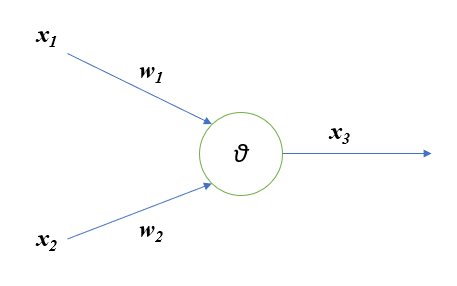
\includegraphics[width=0.6\textwidth]{NeuralNetwork/Schwellenwertelement}
		\caption{Darstellung eines Neurons als einfaches Schwellenwertelement} 
		\label{Schwellenwertelement}
	\end{center}
\end{figure}

\subsection{Gewichte} \label{Gewichte}
Um unterschiedliche Beziehungen zwischen den Aktivierungen der Neuronen abbilden zu können, werden die 
Informationsflüsse zwischen den Neuronen unterschiedlich gewichtet. Zusätzlich können konstante Eingabewerte 
für eine neuronen-spezifische Verzerrung (Bias) sorgen, deren Gewichtung unter Umständen ebenfalls zu ermitteln ist. \cite{Moeser:2018}
In der Darstellung des Netzes als gerichteter Graph werden die Gewichte für gewöhnlich an den Kanten angegeben. 
Mathematisch ist die Darstellung als Matrix üblich. Ein Beispiel für die Darstellung im Graph und die äquivalente Gewichtsmatrix ist in 
Abbildung \ref{Gewichtsmatrix} zu sehen. Die Gewicht werden häufig per Konvention mit zuerst dem Index des Neurons, das das 
Signal als Eingang erhält, und danach dem Index des sendenden Neurons benannt.

\begin{figure}[H]
	\begin{center}
		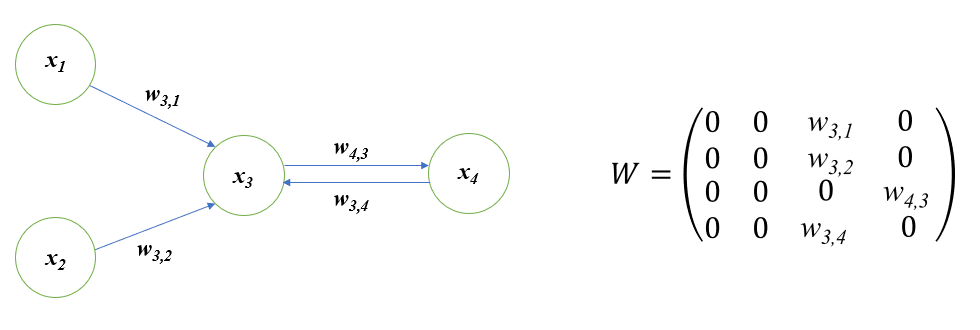
\includegraphics[width=1\textwidth]{NeuralNetwork/Gewichtsmatrix}
		\caption{Graph mit gewichteten Kanten und äquivalente Gewichtsmatrix} 
		\label{Gewichtsmatrix}
	\end{center}
\end{figure}

Zu Beginn werden die Gewichte auf zufällige Werte gesetzt. Üblicherweise werden Werte zwischen -1 und 1 gewählt, 
wobei die aus dem Training resultierenden Werte auch außerhalb dieses Intervalls liegen können. \cite{Moeser:2018} 
Bei bestimmten(!) Trainingsmethoden ist auch eine Initialisierung mit Nullen denkbar. \cite{Kononenko:2007}

\subsection{Bias}

Als Bias wird die neuronenspezifische Verzerrung beschrieben, die als zusätzliche Eingabe
mit konstantem Wert interpretiert werden kann. Der Bias-Wert kann sowohl explizit oder
als Gewichtung eines zusätzlichen konstanten Eingabewert modelliert werden und das
Ergebnis eines Neurons verstärken oder Abschwächen. \cite{Ziegler:2015}

\subsection{Aktivierungs- und Ausgabefunktion} \label{Aktivierungs- und Ausgabefunktion} 
Welchen Wert ein Neuron weitergibt, hängt von den eingehenden Signalen, deren Gewichtung, 
der Aktivierungsfunktion und der Ausgabefunktion ab. Aus den eingehenden Ausgabesignalen 
der verbundenen Neuronen (und evtl. der Rückführung des eigenen Ausgabesignals des betrachteten Neurons selbst) 
berechnet die Aktivierungsfunktion $f$ unter Berücksichtigung der Gewichtung der Signale das 
Aktivitätsniveau des Neurons. \cite{Kruse:2015} 
Der Output des Neurons $x_i$ berechnet sich aus den mit $w_{ij}$ gewichteten eingehenden Signalen 
der $n$ Neuronen $x_j$ mit $j = 1...n$ \\

\begin{center}
$x_i = f(\sum \limits_{j=1}^n w_{ij} x_j)$
\end{center}

Im einfachsten Fall ist die Aktivierungsfunktion linear, dann werden die Signale gewichtet addiert und eventuell mit einem 
konstanten Faktor skaliert. Komplexere, nichtlineare Zusammenhänge können unter Verwendung linearer Aktivierungsfunktionen 
nur in mehrschichtigen Netzen modelliert werden.\cite{Kononenko:2007} Nicht-lineare Funktionen erleichtern die Verallgemeinerung 
und Anpassung an vielfältige Daten und finden daher häufig Verwendung. \cite{Gupta:2020b}

Aus dem so ermittelten Aktivitätsniveau des Neurons wird anschließend unter Zuhilfenahme der Ausgabefunktion der Ausgabewert des 
Neurons bestimmt. In den meisten Fällen wird als Ausgabefunktion die Identität genutzt \cite{Beck.2018}, sodass oft nur die Aktivierungsfunktion 
thematisiert und die Ausgabefunktion vernachlässigt wird.\\

\subsubsection{ReLu-Funktion}
Die Rectified Linear Unit Funktion gilt als die am häufigsten verwendete Aktivierungsfunktion. Sie ist definiert als $R(z)=max(0,z)$, d.h. alle 
negativen Werte werden zu Null und alle Werte über Null bleiben unverändert. Dies kann jedoch auch zu Problemen führen, da negative
 Aktivierungen ignoriert und Neuronen deaktiviert werden. Das soll die Leaky ReLu Funktion korrigieren, bei der im negativen Bereich eine geringe 
 Steigung <1 verwendet wird (siehe Abbildung \ref{ReLu}). Beide Funktionen sowie ihre Ableitungen sind monoton. Dies ist von Bedeutung, damit die 
 Aktivierung mit wachsenden Eingabewerten nicht sinken kann. \cite{Gupta:2020b}\cite{AIUnitedRedaktion.20.12.2018}

\begin{figure}[H]
	\begin{center}
		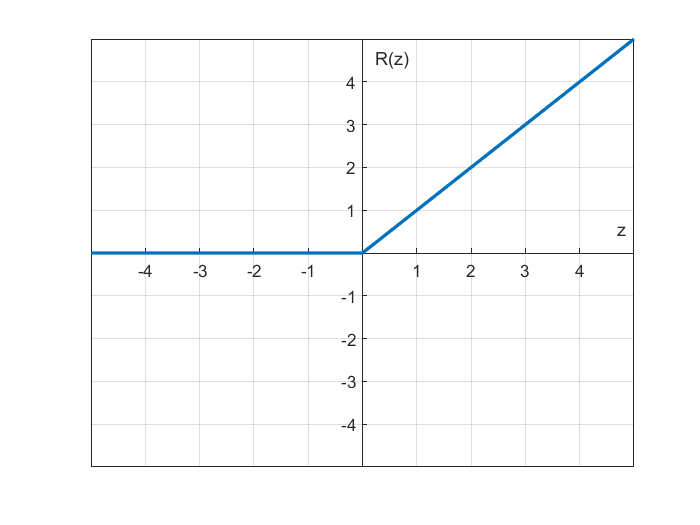
\includegraphics[width=0.49\textwidth]{NeuralNetwork/ReLu}
		\includegraphics[width=0.49\textwidth]{NeuralNetwork/LeakyReLu}
		\caption{ReLu-Funktion (links) und Leaky ReLu} 
		\label{ReLu}
	\end{center}
\end{figure}

\subsubsection{Sigmoid-Funktion} 
Die Sigmoid-Funktion transformiert die Eingangswerte in den Bereich [0,1], siehe Abbildung \ref{Sigmoid}. Die Funktion hierfür lautet 
$S(z)=\frac{1}{1+e^{-z}}$. Durch den Wertebereich ist die Funktion gut zur Darstellung von Wahrscheinlichkeiten geeignet. 
Sie ist immer positiv, sodass die Ausgabe keinen abschwächenden Einfluss auf die nachfolgenden Neuronen haben kann. 
Die Funktion ist differenzierbar und monoton, ihre Ableitung ist jedoch nicht monoton. \cite{Gupta:2020b}\cite{AIUnitedRedaktion.20.12.2018}

\begin{figure}[H]
	\begin{center}
		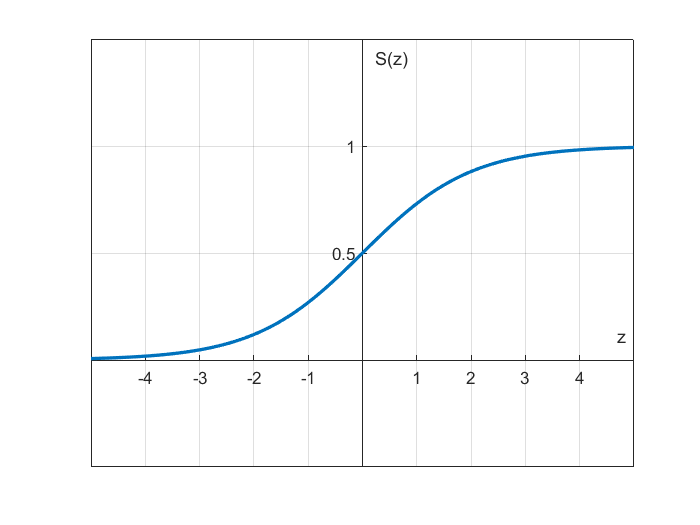
\includegraphics[width=0.6\textwidth]{NeuralNetwork/Sigmoid}
		\caption{Sigmoid-Funktion} 
		\label{Sigmoid}
	\end{center}
\end{figure}

\subsubsection{Softmax-Funktion}
Die Softmax-Funktion wird oft als Überlagerung mehrerer Sigmoid-Funktionen beschrieben. Sie wird vor allem in der Ausgabeschicht verwendet, 
um die Wahrscheinlichkeiten für die verschiedenen Kategorien wiedergeben kann. Der mathematische Ausdruck für die Softmax-Funktion
 lautet wie folgt \cite{Gupta:2020b}:

\begin{center}
$\sigma(z)_j = \frac{e^{z_j}}{\sum\nolimits_{k=1}^K e^{z_k}}$
\end{center}

%Die Softmax-Funktion ist eine Aktivierungsfunktion zur Identifizierung verschiedener Klassen. Es wird die Wahrscheinlichkeitsverteilung jedes Ergebnisses berechnet. Dabei ist die
%	Summe aller möglichen Wahrscheinlichkeiten immer 1. Die einzelnen Wahrscheinlichkeitsbereiche befinden 
%	sich zwischen $0$ und $1$. Die Ausgabe der Softmax-Funktion ist das Verhältnis
%	des Exponentials des Eingabewerts und der Summe der Exponentialwerte. Typischerweise
%	befindet sich die Softmax-Funktion im Output-Layer, kann aber auch in verschiedenen
%	Schichten verwendet werden. \cite{Polamuri:2017}

\subsection{tanh-Funktion}%neu

Die Funktion Tangens Hyperbolicus ist eine nicht-lineare Funktion im Wertebereich von $-1$
bis $1$. Sie ähnelt der Sigmoid-Funktion mit dem großen Unterschied der Punktsymmetie
am Ursprung. Die Funktion ist definiert als:

\begin{center}
  $\tanh(z) = \frac{2}{1 + e^{-2z}} -1$
\end{center}

Die negativen Eingänge sind stark negativ und die Null-Eingänge nahe am Nullpunkt des
Diagramms. Es können negative Ausgaben erfolgen, wodurch auch die gewichtete Summe
eines Neurons des nachfolgenden Layers negativ beeinflusst werden kann. Besonders gut
eignet sich diese Funktion, zur Differenzierung von zwei Klassen. Die Funktion ist differenzierbar,
 monoton und die Ableitung ist nicht monoton. \cite{Gupta:2020b} Die Abbildung~\ref{NNTanh}
zeigt die Funktion Tangens Hyperbolicus im Definitionsbereich von $-6$ bis $6$.

\begin{figure}[H]
	\begin{center}
	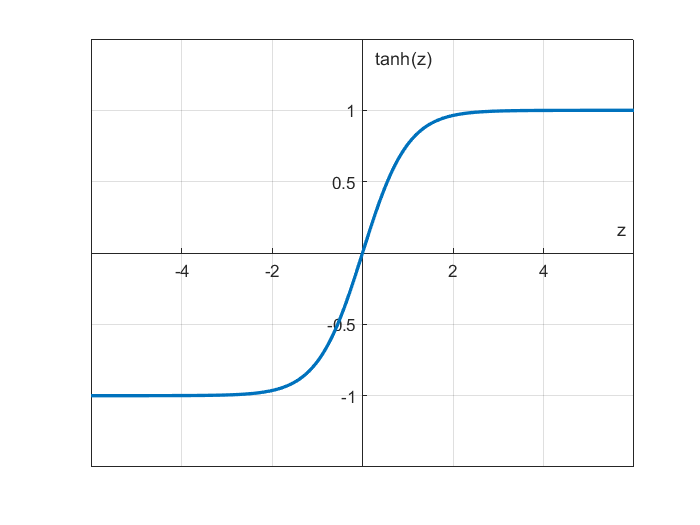
\includegraphics[width=0.6\textwidth]{NeuralNetwork/Tanh}
	\caption{Funktion Tangens Hyperbolicus}\label{NNTanh}
	\end{center}
\end{figure}

	
	

\section{Training}%mögliche Ergänzung: Hebb-Regel (unüberwachtes Lernen)
Die große Stärke neuronaler Netze liegt in der Fähigkeit, zu lernen. Der Lernprozess besteht bei neuronalen Netzen in der Anpassung 
der Gewichte mit dem Ziel, bei entsprechenden Eingabesignalen in die Eingangsschicht den/die gewünschten Ausgabewert/-e in der 
Ausgabeschicht auszugeben. Dafür werden die Gewichte zunächst zufällig initialisiert und dann nach den Lernregeln angepasst.\\


\subsection{Propagation}

Die Propagation bezeichnet den Vorgang bei dem Informationen über den Input-Layer in
das Netz geschickt werden und diese bis zum Output-Layer durchlaufen. Bewegt sich die
Information nur vom Input- zum Output-Layer, wird von einem vorwärts gerichteten Netz
oder auch von der Forwardpropagation gesprochen. Zu Beginn wird dabei die Eingabe in
die Input-Layer kopiert und anschließend an die erste versteckte Schicht geleitet. Welche
Informationen diese Schicht an die nächste weitergibt, hängt von den Gewichtungen und
den Aktivierungsfunktionen ab. Zuletzt kann die Ausgabe am Output-Layer abgelesen
werden. \cite{Kriesel:2008}


\subsection{Fehler}

Als Fehler wird die Abweichung bezeichnet, zwischen der tatsächlichen Netzausgabe und
der gewünschten Netzausgabe, nachdem die Eingabedaten durch das gesamte neuronale
Netz propagiert wurden. \cite{Kriesel:2008}


\subsection{Delta-Regel} 
Grundlage des Lernprozesses ist die Delta-Regel. Für jeden Eingangsdatenpunkt der Lernphase wird die Differenz zwischen 
tatsächlichem und erwartetem (richtigem) Output ermittelt. Dann werden die Gewichte so verändert, dass der Fehler kleiner 
wird. Um die Richtung zu bestimmen, in die die Gewichte verändert werden müssen, wird die Ableitung der Fehlerfunktion 
genutzt (Gradientenabstieg). Die Stärke der Anpassung wird durch die Lernrate bestimmt. Dieser Vorgang wird iterativ wiederholt, 
bis das Abbruchkriterium, z.B. ein genügend kleiner Fehler, erfüllt ist.\cite{Kononenko:2007}\\

\begin{center}
$\Delta w_{ij} = \varepsilon  (x_i - l_i)  f'(\sum_{j} w_{ij} x_j) $
\end{center}

Diese Regel kann unmittelbar nur auf die Gewichte zwischen der Ausgabeschicht und der ihr vorgelagerten Schicht angewendet 
werden. Für die davorliegenden Schichten muss der Fehler rückwärts durch das Netz propagiert werden, 
da die gewünschten Ausgaben für die versteckten Netze nicht gegeben sind. \cite{Kruse:2015} \\

\subsection{Fehler-Rückübertragung (Backpropagation)} 
Im Verfahren der Fehler-Rückübertragung (Backpropagation) wird aus der Änderung der Neuronen in der höheren 
Schicht rekursiv die Änderung der Werte der verdeckten Neuronen berechnet. Dafür muss zunächst die Netzausgabe 
berechnet werden (Vorwärtspropagieren). Der erhaltene Fehler wird beim Rückwärtspropagieren verwendet, um die 
Gewichte von Schicht zu Schicht anzupassen. Dieser Prozess wird auf alle Trainingsdaten angewendet, 
bis das Abbruchkriterium erfüllt ist. \cite{Ertel:2016}

Dieses Verfahren ist zum Training neuronaler Netze etabliert. Dennoch gibt es einige Schwierigkeiten, 
die berücksichtigt werden müssen. Beispielsweise kann ein lokales Minimum des Fehlers gefunden werden, 
das nicht mehr verlassen wird, sodass das globale Minimum nicht gefunden werden kann. Dieses Problem kann 
abgeschwächt werden, indem das Verfahren mit verschiedenen Startwerten durchlaufen wird. \cite{Kruse:2015}
	
\subsection{Problem des Overfitting}

Wird ein neuronales Netz wiederholt mit bekannten Datensätzen trainiert, kann es vorkommen, 
dass das Netz die Daten auswendig lernt, anstatt ein abstraktes Konzept zu
entwickeln. Dieser Zustand wird als Overfitting bezeichnet. Aus diesem Grund sollen nicht
alle Daten zum Trainieren verwendet werden. Es ist sinnvoll eine Validierungsmenge und
eine Testmenge zurückzuhalten. \cite{Becker:2018}

	
	
\subsection{Epochen, Batches und Steps}

Als Epoche wird ein kompletter Durchlauf aller Input-Daten, mit der Messung des Fehlers, 
sowie die Backpropagation zur Anpassung der Gewichte, bezeichnet. Bei großen Datensätzen 
können die Input-Daten in gleichgroße Gruppen, die sogenannten Batches unterteilt werden. 
So kann ein neuronales Netz schneller trainiert werden. Wichtig dabei ist eine Normalverteilung 
der Werte innerhalb jedes Batches. Wird beispielsweise ein Datensatz von 2.000 Bildern in 
Batches mit jeweils 10 Bildern unterteilt, durchläuft die Epoche 200 Steps. Alternativ kann 
auch die Anzahl der Steps vorgegeben und die Batchgröße entsprechend anpassen werden.\cite{Becker:2018c}

\subsection{Dropout}

Beim Dropout werden einige Neuronen deaktiviert, indem bei der Forwardpropagation ein
definierter Prozentsatz der Neuronen mit Null multipliziert wird. Diese Neuronen haben
dadurch keinen Einfluss mehr auf nachfolgende Aktivierungen. Die Deaktivierung erfolgt
pro Durchlauf auf zufälliger Basis. Ist ein Neuron auf ein Merkmal geprägt und fällt aus,
so lernen die umliegenden Neuronen mit diesem Problem umzugehen. Hierdurch erhöht
sich die Generalisierung des Netzes, es lernt abstraktere Konzepte. Ein Nachteil ist die
Erhöhung der Trainingszeit, da die Parameterrückführung verrauscht ist. Am Ende des
Trainings werden alle Neuronen wieder aktiviert. \cite{Becker:2018c}

\subsection{Korrektklassifizierungsrate und Verlustfunktion}

Die Korrektklassifizierungsrate misst die Fähigkeit des Netzes, Datenpunkte der richtigen
Klasse zuzuordnen. Im Gegensatz hierzu steht die Verlustfunktion. \cite{Chollet:2018}

Beide werden oft während des Trainingsverlaufs dokumentiert, um Rückschlüsse
auf den Trainingsverlauf zu erlauben und Probleme wie overfitting oder zu geringe Anzahlen an Durchläufen
zu erkennen.

\subsection{Trainingsdaten, Validierungsdaten und Testmenge}
	Die Trainingsdaten werden aktiv genutzt, um dem Netz die Merkmale der Klassifizierungen beizubringen. 
	Die Validierungsdaten werden am Ende jeder Epoche dem Netz
	zugespielt, um zu testen wie genau das Netz arbeitet. Auch wenn die Validierungsmenge
	nicht aktiv zum Trainieren verwendet wird, fließen teilweise Information zurück ins Netz.
	Aus diesem Grund wird eine Testmenge verwendet, die nicht mit dem Training des neuronalen Netzes in 
	Verbindung steht und nur den Zweck hat die theoretische Genauigkeit
	des Netzes zu überprüfen. \cite{Becker:2018}

\subsection{Transfer Learning}
	Transfer Learning bedeutet die Übertragung der Ergebnisse eines fertigen neuronalen Netzes auf eine neue Aufgabe. 
	Es können Layer konstant gehalten und nur der Output-Layer
	neu trainiert werden oder mehrere Layer auf Basis des aktuellen Trainingstands nach
	trainiert werden. Werden mehrere oder alle Layer neu trainiert, wird als Startpunkt die
	Gewichtungen des trainierten Netzes verwendet. Welche Strategie genutzt werden sollte
	hängt von zwei Faktoren ab:
	
	\begin{itemize}
		\item Ähnlichkeit der Daten
		\item Größe des neuen Datensatzes
	\end{itemize}
		
	Bei einer hohen Ähnlichkeit der Datensätze bietet das Transfer Learning eine gute Möglichkeit
	um ein neuronales Netz zu verbessern. Ähnlichkeiten bestehen beispielsweise bei einem
	trainierten Netz zur Erkennung von Hunderassen, welches auch für die Erkennung von
	Katzenrassen geeignet wäre. Zur Erkennung von verschiedenen Automodellen wäre dieses Netz jedoch ungeeignet, 
	da zu große Abweichungen der Grundstrukturen vorhanden	wären.
	Bei dem Aspekt der Größe des Datensatz gilt, dass ein Transfer Learning besonders bei
	kleinen Datensätzen geeignet sein kann, da es sonst schnell zu Überanpassung kommt. \cite{Becker:2018}
	
	
\section{Convolutional Neural Networks}
Komplexe Aufgaben wie Muster- und Objekterkennungen mit hochdimensionalen Datensätzen führen bei konventionellen 
Ansätzen zu Konvergenzproblemen und hohen Rechenzeiten. Solche Aufgabenstellungen können mit Algorithmen des 
Deep Learnings gelöst werden. Zu dieser Klasse gehören\ac{cnn}. \cite{Ertel:2016}
Sie können Aufgaben mit weniger Vorverarbeitung als bei anderen Klassifizierungsalgortihmen üblich lösen. 
Zudem müssen die verwendeten Filter nicht selbst designed werden, sondern werden während des Trainings vom Netz 
selbst erlernt. \cite{Saha:2018}

Nach \cite{Sharma:2018}, war eine der ersten erfolgreichen Implementierungen von \ac{cnn}s die Erkennung von 
handgeschriebenen Ziffern im Jahr 1998, die in dem Paper \glqq Gradient-Based Learning Applied to Document Recognition\grqq \cite{LeCun:1998} 
beschrieben wird. Mittlerweile haben sich \ac{cnn}s auf vielen Anwendungsgebieten beweisen können. Die typische Anwendung für \ac{cnn}s ist die Verarbeitung von Daten, die eine bekannte Netzwerk-Topologie. So können sie Objekte in Bildern oder Muster in 
Zeitreihen erkennen. \cite{Namatevs.2017}
Neben der Bildklassifizierung, Objekterkennung und -tracking sind auch Text-, Sprach- und Gestenerkennung typsiche Anwendungen, 
die \cite{Gu:2018} beschreibt. Aber auch in der Industrie zur Defekterkennung finden \ac{cnn}s Einsatz. \cite{LopezdeLacalle:2020}

Im Allgemeinen sind \ac{cnn}s aus den Bausteinen Convolutional Layer, Pooling Layer und Fully Connected Layer aufgebaut, wobei für 
gewöhnlich jeder Baustein mehr als ein Mal verwendet wird. Im Folgenden werden diese Bausteine beschrieben. Dabei wird primär 
von der Verwendung von \ac{cnn}s zur Bildklassifizierung ausgegangen.

\subsection{Convolutional Layer}
Hauptkomponente des \ac{cnn} sind Filter, die in der Convolutional Layer auf die Eingangsdaten/-bilder angewendet werden. 
Als Eingabe erhält die Convolutional Layer einen n-dimensionalen Tensor, beispielsweise ein Bild mit drei Farbkanälen, und 
wendet mehrere Kernel auf diese an. Durch Faltung von Tensor und Kernel wird das Bild gefiltert. Die Ergebnisse der Faltung 
mit den verschiedenen Filtern werden gestapelt, sodass als Ergebnis wieder ein Tensor ausgegeben wird. \cite{Michelucci:2019}

Die Operation der Faltung zwischen zwei Matrizen bzw. Tensoren bedeutet die Addition der Produkte aus der Multiplikation der jeweils 
korrespondierenden Elementen beider Matrizen bzw. Tensoren. Da die Faltung in der Convolutional Layer aber für gewöhnlich zwischen 
einem Tensor mit vielen Einträgen und einem dagegen kleinen Kernel stattfindet, muss die Faltung für einzelne Teile des Eingangstensors 
separat durchgeführt werden. Dabei beginnt man für gewöhnlich mit den ersten Einträgen oben links und verschiebt bildlich gesprochen 
den Kernel nach der ersten Faltung relativ zum Eingangstensor um eine bestimmte Anzahl an Spalten und berechnet die Faltung erneut. 
Ist man damit am rechten Rand angelangt, wird der Kernel in der Zeile verschoben und der Vorgang wiederholt. Der als Stride bezeichnete 
Wert gibt an, um wie viele Spalten und Zeilen der Kernel jeweils relativ zum Eingangstensor verschoben wird. Zusätzlich wird für gewöhnlich 
für jeden berechneten Pixel eine Aktivierungsfunktion angewendet. \cite{Michelucci:2019}\\

Bei diesem Vorgang wird aus einem Tensor mit den Dimensionen $h_1 \times w_1 \times d_1$ und den Kerneln mit jeweils 
der Dimension $h_2 \times w_2 \times d_1$, die gestapelt werden zu den Dimensionen $h_2 \times w_2 \times d_2$, 
ein Ausgabetensor mit den Dimensionen $h_3 \times w_3 \times d_2$. \cite{Arunava:2018}

Dabei hängen $h_3$ und $w_3$ von Höhe und Breite des Eingangstensors sowie der Filter und dem gewählten Stride ab, 
während $d_2$ durch die Anzahl an Filtern gegeben ist.

Wenn die Größe des Eingangstensors, des Kernels und des Strides nicht entsprechend zueinanderpassen, können Pixel 
am Rand des Bildes nach dem oben beschriebenen Vorgehen nicht erreicht werden. Deshalb werden manchmal zusätzliche 
Pixel hinzugefügt. Man spricht hier von Padding, bzw.von Zero-Padding, da die hinzugefügten Pixel meist mit dem Wert Null 
gefüllt werden. \cite{Michelucci:2019}

Die Parameter, die in einem \ac{cnn} gelernt werden sind die Filter selbst. Für $k$ Filter der Dimension $m \times n$ 
müssen unter Berücksichtigung von einem Biasterm pro Filter insgesamt $k \cdot m \cdot n + k$ Parameter gelernt werden. 
Bemerkenswert ist dabei, dass diese Zahl unabhängig von der Größe des Eingangsbildes ist, während in konventionellen 
Feed-Forward Netzen die Anzahl der Gewichte von der Größe des Inputs abhängt.\cite{Michelucci:2019}\\

Die Convolutional Layer muss nicht unbedingt die erste Schicht sein, sondern kann auch vorverarbeitete Daten 
als Input erhalten. Meist werden mehrere Convolutional Layers verwendet.\cite{Michelucci:2019}\\
Die Filter der ersten Convolutional Layer detektieren Merkmale auf niedriger Ebene wie Farben, Kanten und Kurven, 
während in höheren Schichten abstraktere Merkmale erkannt werden. Durch das Stapeln mehrerer Convolutional 
und Pooling Layers können nach und nach Merkmalsdarstellungen auf höherer Ebene extrahieren werden. 
Zudem wird auch die Dimensionalität fortlaufend reduziert, was den Berechnungsaufwand reduziert. 
\cite{Gu:2018} \cite{Saha:2018}

\subsection{Pooling Layer}%auch: Mixed, Stochastic, Spectral Pooling
In der Regel folgt auf jede Convolutional Layer eine Pooling Layer. Manchmal werden beide zusammen 
als eine Schicht bezeichnet, da in der Pooling-Schicht keine Gewichte gelernt werden. \cite{Michelucci:2019}

Sie reduziert die Auflösung der vorherigen Feature-Maps durch Komprimierung und reduziert so die 
Komplexität und damit Berechnungsaufwand. Zudem wird das Netz so robuster gegenüber kleinen 
Variationen der erlernten Merkmale und konzentriert sich auf die wichtigsten Muster. \cite{Namatevs.2017}

Es gibt verschiedene Arten des Poolings. Am verbreitesten sind das Maximum und Average Pooling. 
Beim Maximum Pooling wird aus jedem vom Kernel abgedeckten Abschnitt des Tensors nur der Maximalwert gespeichert. 
Beim Average Pooiling hingegen wird für jeden Abschnitt der Durchnschnittswert ermittelt. \cite{Saha:2018}

Die Pooling-Schicht bringt keine neuen lernbaren Parameter mit sich, dafür jedoch zwei neue Hyperparameter, 
nämlich die Dimension des Kernels und den Stride. \cite{Michelucci:2019}

\subsection{Fully Connected Layer}
Nach mehreren Convolutional und Pooling Layers wird das Bild zu einem einzelnen Vektor ausgerollt (engl. flatten). 
Diese Ausgabe wird in ein neuronales Feed-Forward-Netzwerk eingespeist (je Eintrag im Vektor ein Neuron). 
Dieses ist vollständig vernetzt und so in der Lage, die nicht-linearen Zusammenhänge aus den herausgearbeiteten 
Merkmalen zu extrahieren und so zu einer Klassifizierung zu gelangen.\cite{Saha:2018}

Als Aktivierungsfunktion wird meist die ReLu-Funktion verwendet. In der Ausgabeschicht findet die Softmax-Funktion verwendet, 
um die Wahrscheinlichkeiten der einzelnen zuzuordnenden Klassen wiederzugeben. \cite{Arunava:2018}

\subsection{Hyperparameter}
Beim Aufbau und/oder Training eines \ac{cnn} müssen verschiedene Parameter berücksichtigt werden. 
Es muss die Architektur des Netzes und die Reihenfolge der Schichten festgelegt werden. 
Es gibt neue Ansätze zu verschiedenen Faltungsverfahren, aus denen ausgewählt werden kann. 
Außerdem müssen die Größe und Anzahl der Filter und der Stride festgelegt werden. 
Auch das Pooling-Verfahren muss definiert werden, sowie die Aktivierungsfunktionen in den vollvernetzten Schichten.\Mynote{vollvernetzt? Text verbessern} 
Ebenso muss definiert werden, wie viele Neuronen die Eingangsschicht haben soll (dies beeinflusst die mögliche Bildgröße) 
und aus wie vielen Schichten und Neuronen je Schicht die Fully Connected Layer aufgebaut sein soll.

Viele Überlegungen müssen bezüglich der Datenbank gemacht werden. Die Komplexität des zu trainierenden Netzes 
hängt vor allem davon ab, ob nur ein Eingangskanal (schwarz-weiß oder Graustufen) genutzt wird oder drei (RGB). 
Soll zur Reduzierung der Komplexität nur ein Farbkanal verwendet werden, müssen die Bilder entsprechend vorbereitet werden. 
Ebenso muss eventuell die Größe (Anzahl Pixel, Höhe und Breite) der Bilder angepasst werden, sodass sie zur verwendeten Architektur passt. 
Auch eine Normalisierung der Bilder kann hilfreich sein.

Da die Bilder dem neuronalen Netz als Datenarrays präsentiert werden, spielt das Dateiformat keine direkte Rolle. 
Indirekt können aber die verschiedenen Bildqualitäten der verschiedenen Formate die Performance der Netze beeinflussen. 
So können zum Beispiel mit hochauflösenden Bildern trainierte Netze schlechte Resultate liefern, wenn sie komprimierte Bilder 
klassifizieren sollen. \cite{Dodge:2016}Auch durch die verschiedenen Komprimierungen können Unterschiede entstehen,
 sodass verschiedenen Dateiformate nicht gemischt werden sollten.

\subsection{Feinabstimmung}

	Bei der Feinabstimmung können bestimmte Layer aus der Faltungsebene gezielt trainiert
	werden. Mit einer geringen Anzahl von Trainingsbildern kann das Netz gut auf eine neue
	Aufgabe übertragen werden. Dies geht deutlich schneller als ein neuronale Netz von Grund
	auf neu zu entwerfen. \cite{Chollet:2018}		

\subsection{Merkmalsextraktion}

Bei der Merkmalsextraktion werden aus einem trainierten \ac{cnn} die Faltungsebenen (Convolutional-Layer und Pooling-Layer) 
extrahiert und ein neuer Klassifizierer, also eine vollständig verbundene Schicht mit neuen Klassifizierungen, hinzugefügt. 
Hierbei treten zwei Probleme auf:

\begin{itemize}
	\item Die Repräsentation enthält lediglich Informationen über die Wahrscheinlichkeit des
	Vorkommens der im Grundmodell trainierten Klasse.
	\item  Die voll verbundene Schicht enthält keine Informationen darüber, wo sich das Objekt
	befindet.
\end{itemize}
	
	Sollte die Position eines Objektes im Bild eine Rolle spielen, sind die voll verbundenen
	Schichten weitgehend unbrauchbar, da die späteren Layer nur abstrakte Konzepte erzeugen. \cite{Chollet:2018}

\subsection{AlexNet}
Die populärsten \ac{cnn}s für Objektdetektierung und -klassifizierung aus Bilddaten sind AlexNet, GoogleNet und ResNet50. \cite{Sharma:2018}

Gu et al. \cite{Gu:2018} bezeichnen die Entwicklung von AlexNet im Jahr 2012 als Durchbruch der Bildklassifizierung im großen Maßstab. 
Nichtsdestotrotz ist seine Architektur nur so komlpex, dass die Funktionsweise nachvollziehbar bleibt. Daher scheint es eine gute Wahl für erste Versuche eines eigenen Trainings zu sein.


AlexNet besteht aus fünf Convolutional Layers und drei Fully Connected Layers. Anzahl und Größe der Filter sowie ihr Stride sind 
der Übersichtlichkeit halber in Tabelle \ref{ConvAlex} dargestellt.
Nach der ersten und zweiten Faltungsschicht folgt je eine Response-Normalization Layer, auch als Batch-Normalisierung bezeichnet. 
Diese zuätzliche Schicht soll durch Normalisierung die Auswirkung instabiler Gradienten mildern.
Nach den Response-Normalization Layers als auch nach der fünften Convolutional Layer folgt eine Max-Pooling Layer. 
Als Pooling-Methode wurde Overlapping-Pooling gewählt. Das bedeutet, dass sich die einzelnen Abschnitte, auf die das Pooling angewendet wird, 
überlappen. Der Pooling-Bereich misst 3x3 und der Stride 2 pixel.
Auf die Ausgabe jeder Convolutional Layer und jeder der vollständig vernetzten Schichten wird die ReLu-Funktion angewendet.
Jede Fully Connected Layer besteht aus 4096 Neuronen. Die Ausgabeschicht nutzt die Softmax-Funktion um über die Ausgabeneuronen die 
Wahrscheinlichkeiten für die verschiedenen Kategorien abzubilden. \cite{Krizhevsky:2012}\cite{Alake:2020}

\begin{table} [H]
\centering
	\begin{tabular} {l l l l l}
Convolutional Layer & Anzahl Kernel & Dimension & Stride \\ \hline
1 & 96 & $11\times11\times3$ & 4\\
2 & 256 & $5\times5\times48$ & 1\\
3 & 384 & $3\times3\times256$ & 1\\
4 & 384 & $3\times3\times192$ & 1\\
5 & 256 & $3\times3\times192$ & 1\\
\end{tabular}
\caption{Spezifikationen der Convolutional Layer}
\label{ConvAlex}
\end{table}

Insgesamt besteht AlexNet aus 650000 Neuronen. Es müssen etwa 60 Millionen Paramter trainiert werden. \cite{Krizhevsky:2012}

Damit liegt es etwa im Mittelfeld verglichen mit der Anzahl lernbarer Parameter in anderen erfolgreichen \ac{cnn}s.


Die Eingabebilder für AlexNet müssen auf die Größe $227 \times 227$ zugeschnitten werden. Es werden drei Farbkanäle verwendet 
(siehe Tabelle \ref{ConvAlex}), daher ist keine Konvertierung zu Graustufen notwendig, jedoch normalisiert man die Daten für 
gewöhnlich auf den Mittelwert 0 und Standardabweichung 1.\cite{Alake:2020}\\

	
\subsection{YOLO}
Bei YOLO (\textbf{Y}ou \textbf{O}nly \textbf{L}ook \textbf{O}nce) handelt es sich um ein 
State-of-the-Art Echtzeit-Objekterkennungssystem, das Klassifizierung
und Lokalisierung (mit Bounding Box) wesentlich schneller durchführt als konventionelle Systeme.\cite{Redmon.17.02.2021}

Die Detektierung (im Sinne von Klassifizierung UND Lokalisierung) von Objekten ist komplexer als die reine Klassifizierung.
In konventionellen Systemen wird das Bild in viele Regionen aufgeteilt, für die jeweils eine Klassifizierung durchgeführt wird,
um die Regionen zu bestimmen, die das erkannte Objekt enthalten. \cite{Chablani:2017}

Bei YOLO hingegen wird das gesamte Bild einmal in ein einzelnes neuronales Netz gegeben, welches das Bild selbst in einzelne Regionen zerlegt,
wobei für jede dieser Regionen selbst Bounding Boxes und Klassifizierungswahrscheinlichkeiten ermittelt und die Bounding Boxes
mit den Wahrscheinlichkeiten gewichtet werden.

\begin{figure}[H]
	\begin{center}
		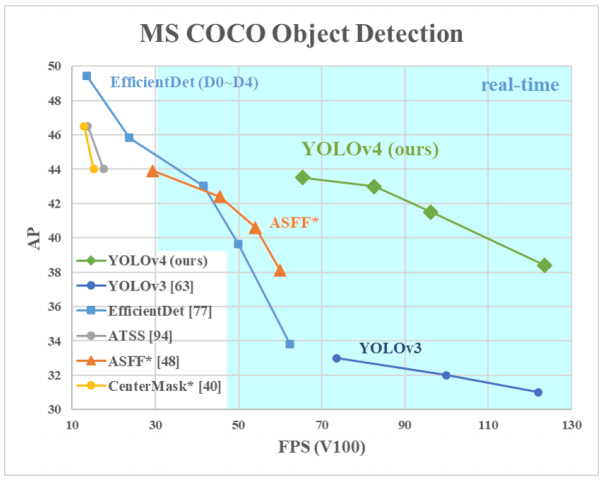
\includegraphics[width=1\textwidth]{NeuralNetwork/YOLO}
		\caption{Das YOLO-System} 
		\label{YOLO}
	\end{center}
\end{figure}

Die Netzarchitektur von YOLO basiert auf GoogLeNet. Es besteht aus 24 Faltungsschichten gefolgt von zwei vollständig vernetzten Schichten. Die ersten
20 Faltungsschichten werden mit dem ImageNet-Datensatz über eine Dauer von einer Woche vortrainiert. Die Bilder in ImageNet haben eine Auflösung von 
224 $\times$ 224, das finale YOLO-Netz nimmt Bilder mit einer Auflösung von 448 $\times$ 448 als Input. Auch das Training findet stets mit den gesamten Bildern
statt, ohne vorherige Unterteilung. \cite{Redmon.08.06.2015}\\

Der Vorteil von YOLO liegt vor allem in seiner Geschwindigkeit, die eine Verarbeitung eines Videostreams mit einer Latenz von weniger als 25 ms erlaubt.
Das macht YOLO 1000 $\times$ schneller als R-\ac{cnn} und 100 $\times$ schneller als Fast R-\ac{cnn}. Da dem Netzwerk das gesamte Bild präsentiert wird und nicht nur 
einzelne Teile dessen, können kontextuelle Informationen berücksichtigt werden. So treten beispielsweise weniger Fehler durch Interpretation von Teilen des
Hintergrunds als Objekt seltener auf als bei anderen Systemen. Außerdem lässt sich das vom System erlernte besser auf andere Gebiete übertragen, sodass etwa
an Fotos gelernte Objekte auch in künstlerischen Darstellungen besser als mit anderen Systemen erkannt werden können.
 \cite{Redmon.08.06.2015} \cite{Redmon.17.02.2021}\\
 
Der YOLO-Code sowie der für das Training verwendete Code sind Open Source.
